\subsubsection*{rsync}
Das Tool \textit{rsync} ist in allen Linux-Distributionen enthalten und insbesondere f�r Scripte einfach verwendbar. Es synchronisiert die Dateien eines Zielverzeichnisses mit dem Quellverzeichnis und �bertr�gt dabei nur die �nderungen. Ein Beispiel zeigt das Sichern der E-Mails und Adressb�cher von Thunderbird:

\begin{verbatim}
   rsync -av --delete $HOME/.thunderbird /backup_dir/.thunderbird
\end{verbatim} 

Eine zweite Variante zum Sichern des gesamten \$HOME inklusive der versteckten Dateien und exklusive eines Verzeichnisses (mp3) mit gro�en Datenmengen:

\begin{verbatim}
   rsync -av --delete --include=$HOME/. --exclude=$HOME/mp3 $HOME /backup_dir/
\end{verbatim} 

Die Option \textit{--delete} l�scht im Orginal nicht mehr vorhandene Dateien auch in der Sicherungskopie. Weitere Hinweise liefert die Manualpage von rsync.\\

Standardm��ig sichert rsync keine versteckten Dateien und Verzeichnisse, die mit einem Punkt beginnen. Diese Dateien und Verzeichnisse m�ssen mit einem "--include" angegeben werden. Im Beispiel werden alle versteckten Verzeichnisse und Dateien mit gesichert.\\

Ein kleines Script, welches alle n�tigen Verzeichnisse synchronisiert, ist schnell gestrickt. Eine backup-freundliche Struktur im \$HOME-Verzeichnis erleichtert dies zus�tzlich. 

\subsubsection*{Grsync}
GRsync ist ein grafischen Interface f�r rsync. Auch dieses Tool ist in allen Linux/Unix Distributionen enthalten.\\

Nach dem Start kann man mit dem Button ``+`` mehrere Profile f�r verschiedene, wiederkehrende Aufgaben anlegen. Jedem Profil wird ein Quell - und ein Zielverzeichnis sowei die rsync-Parameter zugeordnet. Ein Klick auf die kleine Rakete oben rechts startet die Synchronisation (Bild \ref{abb:grsync1}).

\begin{figure}[htb]
\begin{center}
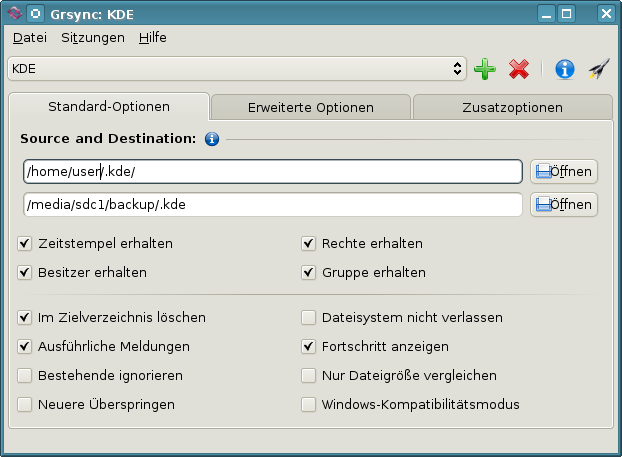
\includegraphics[scale=0.75]{../screenshots/grsync1.png}
\caption{Hauptfenster von Grsync}
\label{abb:grsync1}
\end{center}
\end{figure}